\begin{center}
    \begin{figure}[H]
        \centering

        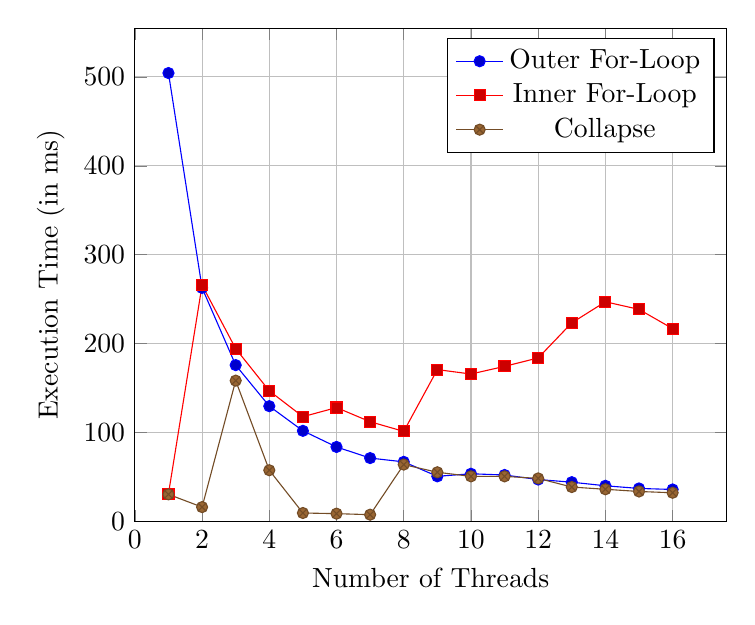
\begin{tikzpicture}
            \begin{axis}[
                title={},
                width=0.75\textwidth,
                xlabel={Number of Threads},
                ylabel={Execution Time (in ms)},
                xmin=0,
                ymin=0,
                grid=major
            ]
                \addplot coordinates {
                    (1,504.363)(2,262.6)(3,175.732)(4,129.548)(5,101.787)(6,83.6696)(7,71.1456)(8,66.8944)(9,50.6149)(10,53.4979)(11,52.1091)(12,47.0084)(13,44.0151)(14,39.9768)(15,36.9805)(16,35.8334)
                };
                \addlegendentry{Outer For-Loop}

                \addplot coordinates {
                    (1,30.9718)(2,265.722)(3,194.251)(4,146.741)(5,117.723)(6,127.965)(7,112.053)(8,101.16)(9,170.682)(10,165.723)(11,174.331)(12,183.822)(13,223.315)(14,246.996)(15,238.439)(16,216.813)
                };
                \addlegendentry{Inner For-Loop}       

                \addplot coordinates {
                    (1,30.3305)(2,15.9853)(3,158.284)(4,57.4573)(5,9.3502)(6,8.62)(7,7.4556)(8,63.8195)(9,55.1714)(10,50.5752)(11,50.5688)(12,48.2911)(13,38.5529)(14,36.0367)(15,33.5607)(16,32.1147)
                };
                \addlegendentry{Collapse}
            \end{axis}
        \end{tikzpicture}
        \caption{HSV Performance Tests dice.png}
    \end{figure}
\end{center}